%%%%%%%%%%%%%%%%%%%%%%%%%%%%%%%%%%%%%%%%%%%%%%%%%%%%%%%%%%%%%%%%%%%%%%%%%%%%%%% 
% Full instructions available at:
% https://github.com/elauksap/focus-beamertheme

\documentclass{beamer}
\usetheme{focus}

% package for font
\usepackage{fontspec}
\defaultfontfeatures{Mapping=tex-text}  %%如果没有它,会有一些 tex 特殊字符无法正常使用,比如连字符。
\usepackage{xunicode,xltxtra}
\usepackage[BoldFont,SlantFont,CJKnumber,CJKchecksingle]{xeCJK}  % \CJKnumber{12345}: 一万二千三百四十五
\usepackage{CJKfntef}  %%实现对汉字加点、下划线等。
\usepackage{pifont}  % \ding{}
% package for math
\usepackage{amsfonts}
% package for graphics
\usepackage[americaninductors,europeanresistors]{circuitikz}
\usepackage{tikz}
\usetikzlibrary{plotmarks}  % placements=positioning
\usepackage{graphicx}  % \includegraphics[]{}
\usepackage{subfigure}  %%图形或表格并排排列
% package for table
\usepackage{colortbl,dcolumn}  %% 彩色表格
\usepackage{multirow}
\usepackage{multicol}
\usepackage{booktabs}
% package for code
\usepackage{fancyvrb}
\usepackage{listings}
% setting for font
%%\setCJKmainfont{Adobe Kaiti Std}
\setCJKmainfont{SimSun}
%%\setCJKmainfont{Microsoft YaHei}
%%\setCJKmainfont{FangSong_GB2312} 
%%\setmainfont{Times New Roman}
%\setsansfont[Mapping=tex-text]{Adobe Song Std}
%如果装了Adobe Acrobat,可在font.conf中配置Adobe字体的路径以使用其中文字体。
%也可直接使用系统中的中文字体如SimSun、SimHei、微软雅黑等。
%原来beamer用的字体是sans family;注意Mapping的大小写,不能写错。
%设置字体时也可以直接用字体名,以下三种方式等同:
%\setromanfont[BoldFont={黑体}]{宋体}
%\setromanfont[BoldFont={SimHei}]{SimSun}
%\setromanfont[BoldFont={"[simhei.ttf]"}]{"[simsun.ttc]"}

% font setting by xeCJK
\setCJKfamilyfont{NSimSun}{NSimSun}
\newcommand{\song}{\CJKfamily{NSimSun}}
%%%\setCJKfamilyfont{AdobeSongStd}{Adobe Song Std}
%%%\newcommand{\AdobeSong}{\CJKfamily{AdobeSongStd}}
\setCJKfamilyfont{FangSong}{FangSong_GB2312}
\newcommand{\fang}{\CJKfamily{FangSong}}
%%%\setCJKfamilyfont{AdobeFangsongStd}{Adobe Fangsong Std}
%%%\newcommand{\AdobeFang}{\CJKfamily{AdobeFangsongStd}}
\setCJKfamilyfont{SimHei}{SimHei}
\newcommand{\hei}{\CJKfamily{SimHei}}
%%%\setCJKfamilyfont{AdobeHeitiStd}{Adobe Heiti Std}
%%%\newcommand{\AdobeHei}{\CJKfamily{AdobeHeitiStd}}
\setCJKfamilyfont{KaiTi}{KaiTi_GB2312}
\newcommand{\kai}{\CJKfamily{KaiTi}}
%%%\setCJKfamilyfont{AdobeKaitiStd}{Adobe Kaiti Std}
\newcommand{\AdobeKai}{\CJKfamily{AdobeKaitiStd}}
\setCJKfamilyfont{LiSu}{LiSu}
\newcommand{\li}{\CJKfamily{LiSu}}
\setCJKfamilyfont{YouYuan}{YouYuan}
\newcommand{\you}{\CJKfamily{YouYuan}}
\setCJKfamilyfont{FZJingLei}{FZJingLeiS-R-GB}
\newcommand{\jinglei}{\CJKfamily{FZJingLei}}
\setCJKfamilyfont{MSYH}{Microsoft YaHei}
\newcommand{\msyh}{\CJKfamily{MSYH}}

\setbeamerfont{frametitle}{series=\Large\hei} % 修改Beamer标题字体

\graphicspath{{figures/}}  %%图片路径
\renewcommand\figurename{图}

% setting for pdf
\hypersetup{% pdfpagemode=FullScreen,%
  pdfauthor={Xiaodong Wang},%
  pdftitle={Title},%
  CJKbookmarks=true,%
  bookmarksnumbered=true,%
  bookmarksopen=false,%
  plainpages=false,%
  colorlinks=true,%
  citecolor=green,%
  filecolor=magenta,%
  linkcolor=blue,%red(default)
  urlcolor=cyan}

% setting for fontspec
\XeTeXlinebreaklocale "zh"  %%表示用中文的断行
\XeTeXlinebreakskip = 0pt plus 1pt minus 0.1pt  %%多一点调整的空间
%%%%%

% 自定义颜色
\def\Red{\color{red}}
\def\Green{\color{green}}
\def\Blue{\color{blue}}
\def\Mage{\color{magenta}}
\def\Cyan{\color{cyan}}
\def\Brown{\color{brown}}
\def\White{\color{white}}
\def\Black{\color{black}}

\lstnewenvironment{xmlCode}[1][]{% for Java
  \lstset{
    basicstyle=\tiny\ttfamily,%
    columns=flexible,%
    framexleftmargin=.7mm, %
    % frame=shadowbox,%
    % rulesepcolor=\color{cyan},%
     frame=single,%
    backgroundcolor=\color{white},%
    xleftmargin=4\fboxsep,%
    xrightmargin=4\fboxsep,%
    numbers=left,numberstyle=\tiny,%
    numberblanklines=false,numbersep=7pt,%
    language=xml, %
    }\lstset{#1}}{}

\lstnewenvironment{javaCode}[1][]{% for Java
  \lstset{
    basicstyle=\tiny\ttfamily,%
    columns=flexible,%
    framexleftmargin=.7mm, %
    frame=shadowbox,%
    rulesepcolor=\color{cyan},%
    % frame=single,%
    backgroundcolor=\color{white},%
    xleftmargin=4\fboxsep,%
    xrightmargin=4\fboxsep,%
    numbers=left,numberstyle=\tiny,%
    numberblanklines=false,numbersep=7pt,%
    language=Java, %
    }\lstset{#1}}{}

\lstnewenvironment{shCode}[1][]{% for Java
  \lstset{
    basicstyle=\scriptsize\ttfamily,%
    columns=flexible,%
    framexleftmargin=.7mm, %
    frame=shadowbox,%
    rulesepcolor=\color{brown},%
    % frame=single,%
    backgroundcolor=\color{white},%
    xleftmargin=4\fboxsep,%
    xrightmargin=4\fboxsep,%
    numbers=left,numberstyle=\tiny,%
    numberblanklines=false,numbersep=7pt,%
    language=sh, %
    }\lstset{#1}}{}

\newcommand\ask[1]{\vskip 4bp \tikz \node[rectangle,rounded corners,minimum size=6mm,
  fill=white,]{\Cyan \includegraphics[height=1.5cm]{question} \Large \msyh #1};}

\newcommand\wxd[1]{\vskip 4bp \tikz \node[rectangle,minimum size=6mm,
  fill=blue!60!white,]{\White \ding{118} \msyh #1};}

\newcommand\cxf[1]{\vskip 4bp \tikz \node[rectangle,rounded corners,minimum size=6mm,
  fill=purple!60!white,]{\White \ding{42} \msyh #1};}

\newcommand\xyy[1]{\vskip 2bp \tikz \node[rectangle,minimum size=3mm,
  fill=black!80!white,]{\White \msyh\scriptsize #1};}

\newcommand\tta[1]{\vskip 4bp \tikz \node[rectangle,minimum size=6mm,
  fill=blue!60!white,]{\White \ding{118} \msyh #1};}

\newcommand\ttb[1]{\vskip 4bp \tikz \node[rectangle,rounded corners,minimum size=6mm,
  fill=purple!60!white,]{\White \ding{42} \msyh #1};}

\newcommand\ttc[1]{\vskip 2bp \tikz \node[rectangle,minimum size=3mm,
  fill=black!80!white,]{\White \msyh\scriptsize #1};}

\newcommand\homework[1]{\vskip 2bp \tikz \node[rectangle,minimum size=3mm,
  fill=red!80!white,]{\White \ding{45} \msyh\scriptsize 课后小作业 } ; {\kai\small #1}} 

\newcommand\notice[1]{\vskip 4bp \tikz \node[rectangle,rounded corners,minimum size=6mm,
  fill=red!80!white,]{\White \scriptsize \ding{42} \msyh #1};}

\newcommand\samp[1]{\vskip 2bp \tikz \node[rectangle,minimum size=3mm,]{\Mage\msyh \small CODE \ding{231} \Black #1};\vskip -8bp}

\newcommand\codeset[1]{\vskip 2bp \tikz \node[rectangle,minimum
  size=3mm]{\Mage\msyh \small 课程配套代码 \ding{231} \Black
    #1};\vskip -4bp}

\newcommand\pptlink[2]{\vskip 4bp \tikz \node[rectangle,rounded corners,minimum size=6mm,
  fill=blue!70!white,]{\href{run:#1}{\White \scriptsize \msyh 动画演示 #2}};}


\makeatletter
\newcommand{\Extend}[5]{\ext@arrow 0099{\arrowfill@#1#2#3}{#4}{#5}}
\makeatother
%%%%%%%%%%%%%%%%%%%%%%%%%%%%%%%%%%%%%%%%%%%%%%%%%%%%%%%%%%%%%%%%%%%%%%%%%%%%%%% 
\title{\hei JAVA应用与开发\\  集合与映射}
\subtitle{\it 让我们愉快的Coding起来吧...}
\author{王晓东}
\titlegraphic{\vspace{-8em}
\includegraphics[height=10cm]{static/ouc.pdf}\vspace{-6em}} 
\institute{中国海洋大学信息学院计算机系}
\date{\today}

\begin{document}
\begin{frame}
  \maketitle
\end{frame}

\begin{frame}
  \frametitle{学习目标}
  \begin{itemize}
  \item 掌握列表(List)、集(Set)、映射(Map)的概念、层次关系
  \item 熟练应用相关集合容器
  \item 掌握迭代器(iterator)、Enumeration接口等容器操作常用API
  \item 了解集合容器的人为性能提升及线程安全等
  \end{itemize}
\end{frame}

\begin{frame}
  \frametitle{大纲}
  \tableofcontents
\end{frame}

\section{集合概念及分类}

%%% \begin{frame}[fragile]
%%%   \frametitle{集合和数组}
%%%   
%%%   \begin{itemize}
%%%   \item 在编程中,常常需要集中存放多个数据。
%%%   \item 从传统意义上讲,数组是我们的一个很好的选择,前提是我们事先已经
%%%     明确知道我们将要保存的对象的数量。一旦在数组初始化时指定了这个数组
%%%     长度,这个数组长度就是不可变的。
%%%   \item 如果我们需要保存一个可以动态增长的数据(在编译时无法确定具体的
%%%     数量),java的集合类就是一个很好的设计方案了。
%%%   \end{itemize}
%%% \end{frame}

\begin{frame}[fragile]
  \frametitle{集合和数组}

  \tta{面向存放多个数据的需求}
  
  \begin{itemize}[<+-|alert@+>]\hei
  \item 数组用于存放指定长度的数据。
  \item 需要保存可以动态增长的数据(在编译时无法确定具体的
    数量),则需要用到Java的集合类。
  \end{itemize}
\end{frame}

\begin{frame}[fragile] % [fragile]参数使得能够插入代码
  \frametitle{集合类型}

  {\hei\Red 集合就是将若干用途、性质相同或相近的“数据”组合而成一个整体。}

  \pause
  
  \tta{集合类型分类}

  \begin{description}[<+-|alert@+>]
  \item[集] Set集合中不区分元素的顺序,不允许出现重复元素。例如应用于记
    录所有用户名的场合。
  \item[列表] List集合区分元素的顺序,且允许包含重复元素。相当于数据结
    构中的线性表,具体表现为数组和向量、链表、栈、队列等。
  \item[映射] Map中保存成对的“键\ding{213}值”(Key-Value)信息,映射中不能包含重
    复的键,每个键最多只能映射一个值。
  \end{description}

  \pause

  \notice{注意}
  
  {\kai Java集合中只能保存引用类型的数据,实际上存放的是对象的引用而非
    对象本身。Java API中的集合类型均定义在java.util包中。}
\end{frame}

%%%\begin{frame}[fragile]
%%%  \frametitle{对Java集合中只能保存引用类型的数据的说明}
%%%
%%%  Java集合只能存放引用类型数据,它们都是存放引用类型数据的容器,不能存
%%%  放如int、long、float、double等基本类型的数据。
%%%
%%%  \tta{集合存储对象}
%%%
%%%  Java集合中实际存放的只是对象的引用,每个集合元素都是一个引用变量,实
%%%  际内容都放在堆内存或者方法区里面,但是基本数据类型是在栈内存上分配空
%%%  间的,栈上的数据随时就会被收回的。
%%%
%%%  \tta{基本类型数据如何解决呢?}
%%%
%%%  可以通过包装类把基本类型转为对象类型,存放引用就可以解决这个问题。更
%%%  方便的,由于有了自动拆箱和装箱功能,基本数据类型和其对应对象(包装类)
%%%  之间的转换变得很方便,想把基本数据类型存入集合中,直接存就可以了,系
%%%  统会自动将其装箱成封装类,然后加入到集合当中。
%%%
%%%  \notice{自动拆装箱机制}
%%%\end{frame}

\begin{frame}[fragile] % [fragile]参数使得能够插入代码
  \frametitle{集合相关API的关系}

  \begin{figure}
    \centering
    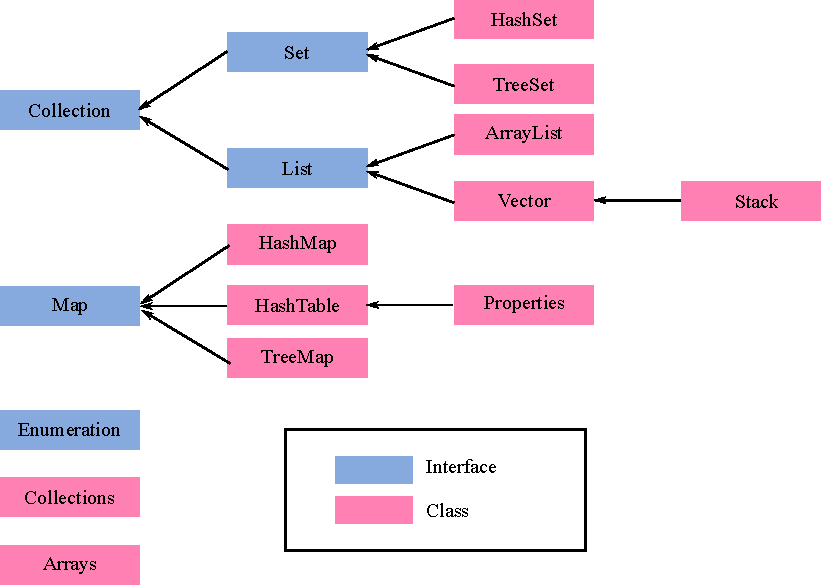
\includegraphics[width=0.8\textwidth]{fig-set-list-map.pdf}
  \end{figure}
\end{frame}


\section{Collection和Map接口}

\begin{frame}[fragile] % [fragile]参数使得能够插入代码
  \frametitle{Collection接口}

  java.util.Collection接口是描述Set和List集合类型(不包含Map)的根接口,
  其中定义了有关集合操作的普遍性方法:
  
  \begin{itemize}[<+-| alert@+>]
  \item boolean add(Object o)\\
    \only<1>{向集合中添加一个元素,在子接口中此方法发生了分化,如Set接口
      中添加重复元素时会被拒绝(返回false,而不是出错);List接口则会接受
      重复元素且返回true。}
  \item boolean remove(Object o) \\
    \only<2>{从集合中移除指定的元素。}
  \item int size()\\
    \only<3>{返回集合中元素的数目。}
  \item boolean isEmpty()\\
    \only<4>{判断集合是否为空(即是否包含任何元素)。}
  \item boolean contains(Object o) \\
    \only<5>{判断集合中是否包含指定的元素。}
  \item void clear()\\
    \only<6>{移除当前集合中的所有元素。}
  \item Iterator iterator()\\
    \only<7>{返回在此集合的元素上进行迭代的迭代器。}
  \item Object[] toArray()\\
    \only<8>{返回包含当前集合中所有元素的数组。}
  \end{itemize}
\end{frame}

\begin{frame}[fragile] % [fragile]参数使得能够插入代码
  \frametitle{Set和List接口}

  \begin{block}{}
    java.util.Set和java.util.List分别描述前述的集和列表结构,二者均
    为Collection的子接口。Set接口模拟了数学意义的集合;List接口规定使用
    者可以对列表元素的插入位置进行精确控制,并添加了根据元素索引来访问
    元素等功能。
  \end{block}

  \pause
  
  \tta{List接口中新添加的方法}

  \begin{itemize}[<+-| alert@+>]\kai
  \item void add(int index, Object element)
  \item Object get(int index)
  \item Object set(int index, Object element) 
  \item int indexOf(Object o) 返回列表中首次出现指定元素的索引,如果列表不包含指定元素,则返回-1。
  \item Object remove(int index)
  \end{itemize}
\end{frame}

\begin{frame}[fragile] % [fragile]参数使得能够插入代码
  \frametitle{Map接口}

  java.util.Map接口描述了映射结构,Map结构允许以{\hei\Blue 键集、值集合
    或键—值映射关系集}的形式查看某个映射的内容。主要方法:
  
  \begin{itemize}[<+-| alert@+>]\kai
  \item Object put(Object key, Object value)\\
    \only<1>{向当前映射中加入一组新的健—值对,并返回所加入元素的“值”,
      如果此映射中以前包含一个该键的映射关系,则用新值替换旧值。}
  \item Object get(Object key)\\
    \only<2>{返回此映射中映射到指定键的值,没有则返回null。}
  \item boolean isEmpty()
  \item void clear()
  \item int size()
  \item boolean containsKey(Object key)\\
    \only<6>{如果映射中包含指定键的映射关系,则返回true,否则返回false。}
  \item boolean containsValue(Object value)
  \item Set keySet()\\
    \only<8>{返回此映射中包含的键的set视图,此Set受映射支持,所以对映射
      的改变可以在此Set中反映出来,反之亦然。}
  \item Collection values()\\
    \only<9>{返回此映射包含值的Collection视图,此Collection受映射支持,
      所以对映射的改变可以在此Collection中反映出来,反之亦然。}
  \end{itemize}
\end{frame}

\section{列表}

\begin{frame}[fragile] % [fragile]参数使得能够插入代码
  \frametitle{ArrayList类}

  java.util.ArrayList类实现了List接口,用于表述长度可变的数组列表。

  ArrayList列表允许元素取值为null。除实现了List接口定义的所有功能外,还提供了一些方法来操作列表容量的大小,相关方法包括:

  \begin{itemize}\kai
  \item public ArrayList()\\构造方法:创建一个初始容量为10的空列表。
  \item public ArrayList(int initialCapacity)
  \item {\Red public void ensureCapacity(int minCapacity)\\对容器进行扩容。}
  \item public void trimToSize() \\将此ArrayList实例的容量调整为列表的当前大小。
  \end{itemize}
\end{frame}

\begin{frame}[fragile]
  \frametitle{代码的局部性能优化 ensureCapacity}

  \wxd{ArrayList ensureCapacity(int n)}

  \begin{itemize}\kai
  \item 该方法可以对ArrayList底层的数组进行扩容。
  \item 显式地调用这个函数,如果参数大于底层数组长度的1.5倍,那么这个数
    组的容量就会被扩容到这个参数值,如果参数小于底层数组长度的1.5倍,那
    么这个容量就会被扩容到底层数组长度的1.5倍。
  \item 在适当的时机,好好利用这个函数,将会使我们写出来的程序性能得到
    很大的提升。
  \end{itemize}

  \codeset{sample.setlistmap.ArrayListEnSureCapacitySample.java}
\end{frame}

\begin{frame}[fragile] % [fragile]参数使得能够插入代码
  \frametitle{Vector类}

  java.util.Vector也实现了List接口,其描述的也是可变长度的对象数组。

  \wxd{与ArrayList的差别}

  {\Red\kai Vector是同步(线程安全)的,运行效率要低一些,主要用在在多线
    程环境中,而ArrayList是不同步的,适合在单线程环境中使用。}

  常用方法(除实现List接口中定义的方法外):

  \begin{itemize}\small
  \item public Vector()
  \item public Object elementAt(int index)
  \item public void addElement(Object obj)
  \item public void removeElementAt(int index)
  \item public void insertElementAt(E obj, int index) 
  \item public boolean removeElement(Object obj) 
  \item public void removeAllElements()
  \item public Object[] toArray()
  \end{itemize}
\end{frame}

\begin{frame}[fragile]
  \frametitle{何谓线程安全}

  \wxd{线程安全的一般意义}

  \begin{description}\kai\small
  \item[线程安全] 在多线程访问时采用加锁机制,当一个线程访问该类的某个
    数据时进行保护,其他线程不能进行访问直到该线程读取完,其他线程才可
    使用,不会出现数据不一致或者数据污染。(Vector、HashTable等)
  \item[线程不安全] 不提供数据访问保护,有可能出现多个线程先后更改数据导致出现“脏数据”。
    (ArrayList、LinkedList、HashMap等)
  \end{description}

  \begin{figure}
    \centering
    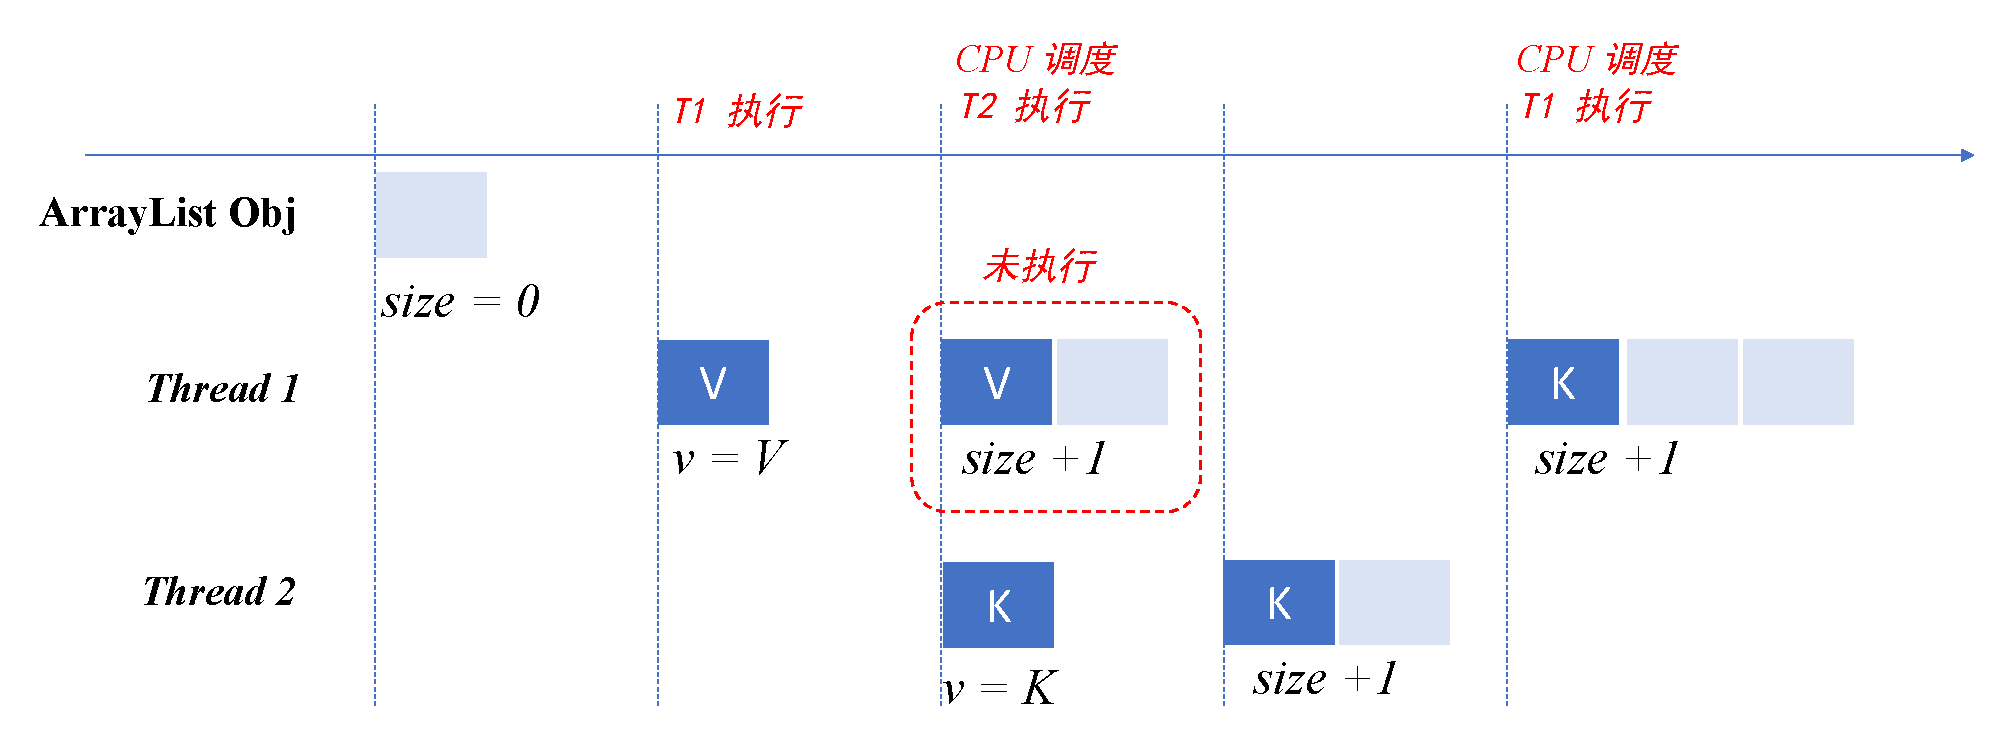
\includegraphics[width=0.85\textwidth]{thread-safe.pdf}
  \end{figure}

  %%% 比如一个 ArrayList 类,在添加一个元素的时候,它可能会有两步来完
  %%% 成:1. 在 Items[Size] 的位置存放此元素;2. 增大 Size 的值。 在单线程
  %%% 运行的情况下,如果 Size = 0,添加一个元素后,此元素在位置 0,而
  %%% 且 Size=1; 而如果是在多线程情况下,比如有两个线程,线程 A 先将元素存
  %%% 放在位置 0。但是此时 CPU 调度线程A暂停,线程 B 得到运行的机会。线
  %%% 程B也向此 ArrayList 添加元素,因为此时 Size 仍然等于 0 (注意哦,我们
  %%% 假设的是添加一个元素是要两个步骤哦,而线程A仅仅完成了步骤1),所以线
  %%% 程B也将元素存放在位置0。然后线程A和线程B都继续运行,都增加 Size 的
  %%% 值。 那好,我们来看看 ArrayList 的情况,元素实际上只有一个,存放在位
  %%% 置 0,而 Size 却等于 2。这就是“线程不安全”了。
\end{frame}

\begin{frame}[fragile] % [fragile]参数使得能够插入代码
  \frametitle{Stack} java.util.Stack类继承了Vector类,对应数据结构中
  以{\hei\Blue “后进先出”(Last in First out, LIFO)方式存储和操作数
    据的对象栈}。Stack类提供了常规的栈操作方法:

  \begin{itemize}\kai\small
  \item public Stack() 构造方法,创建一个空栈。
  \item public Object push(E item) 向栈中压入数据。
  \item public Object pop() 移除栈顶对象并作为此方法的返回值。
  \item public Object peek() 查看/返回栈顶对象,但不从栈中移除它。
  \item public boolean empty() 测试栈是否为空。
  \item public void clear() 清空栈。
  \item public int search(Object o) 返回对象在栈中的位置,以1为基数。
  \end{itemize}
\end{frame}

\section{Iterator接口}

\begin{frame}[fragile] % [fragile]参数使得能够插入代码
  \frametitle{Iterator接口}

  \wxd{统一的遍历方式}
  
  \begin{itemize}
  \item 对于ArrayList可以使用get()方法访问其元素;
  \item 对于Vector,还可以使用elementAt()方法访问其元素;
  \item 后续Set和Map集合也有各自不同的元素访问方式。
  \end{itemize}
  \pause {\Blue\hei 是否有一种统一的方式来遍历各种不同类型集合中的元素呢?}

\end{frame}

\begin{frame}[fragile] % [fragile]参数使得能够插入代码
  \frametitle{Iterator接口}

  Java.util.Iterator接口描述的是以统一方式对各种集合元素进行遍历/迭代的工具,也称为“{\Blue\hei 迭代器}”。

  迭代器允许在遍历过程中移除集合中的(当前遍历到的那个)元素。主要方法包括:

  \begin{itemize}\small\kai
  \item boolean hasNext()\\
    如果仍有元素可以迭代,则返回true,否则返回false。
  \item Object next()\\
    返回迭代的下一个元素,重复调用此方法直到haseNext()方法返回false。
  \item void remove()\\
    将当前迭代到的元素从迭代器指向的集合中移除。
  \end{itemize}
\end{frame}

\begin{frame}[fragile] % [fragile]参数使得能够插入代码
  \frametitle{使用迭代器}

  我们一般不直接创建迭代器对象,而是通过调用集合对象的iterator()方法(该方法在Collection接口中定义)来获取。

  \samp{TestIterator.java}

  \begin{javaCode}
    import java.util.ArrayList;
    import java.util.Iterator;

    public class TestIterator {
      public static void main(String[] args) {
        ArrayList a = new ArrayList();
        a.add("China");
        a.add("USA");
        a.add("Korea");
        Iterator it = a.iterator();
        
        while(it.hasNext()) {
          String country = (String) it.next();
          System.out.println(country);
        }
      }
    }
  \end{javaCode}
  {\kai\Red 注意:迭代器相当于原始集合的一个“视图”,即一种表现形式,而不是复制其中所有元素得到的拷贝,因此在迭代器上的操作将影响到原来的集合。}
\end{frame}

\section{集}

\begin{frame}[fragile] % [fragile]参数使得能够插入代码
  \frametitle{HashSet类}

  java.util.HashSet类实现了java.util.Set接口,描述典型的Set集合结构。

  \begin{itemize}
  \item HashSet中不允许出现重复元素,不保证集合中元素的顺序。
  \item HashSet中允许包含值为null的元素,但最多只能有一个null元素。
  \end{itemize}
\end{frame}

\begin{frame}[fragile] % [fragile]参数使得能够插入代码
  \frametitle{TreeSet类}

  java.util.TreeSet类也实现了java.util.Set,它描述的是Set的一种变体——可以
  实现排序功能的集合。

  \begin{itemize}\kai
  \item 在将对象元素添加到TreeSet集中时会自动按照某种比较规则将其插入到有
    序的对象序列中,以保证TreeSet集合元素组成的对象序列时刻按照“升序”排
    列(例如按照字典顺序排列);
  \item 对于用户自定义的类型的数据可以自行定义其所需的排序规则(使用Comparable接口)。
  \end{itemize}
\end{frame}

\begin{frame}[fragile] % [fragile]参数使得能够插入代码
  \frametitle{Comparable接口}

  java.lang.Comparable接口中定义的compareTo()方法用于提供对其实现类的对象
  进行整体排序所需的比较逻辑,所为的排序可以理解为按照某种标准来比较对象
  的大小以确定其次序。

  \begin{itemize}\kai
  \item 实现类基于compareTo()方法的排序被称为{\Blue 自然排序}。
  \item compareTo()方法被称为它的{\Blue 自然比较方法},具体的排序原则可由实现类根据需要而定。
  \end{itemize}

  \xyy{方法格式}
  \begin{javaCode}
    int compareTo(Object o) {
      
    }   
  \end{javaCode}

  \samp{sample.setlistmap.NatrualOrderingSample.java}
  
\end{frame}

\begin{frame}[fragile] % [fragile]参数使得能够插入代码
  \frametitle{Comparable接口}

  \wxd{使用Comparable接口实现自然排序}
  \samp{Person.java}
  \begin{javaCode}
    public class Person implements java.lang.Comparable {
      private final int id;
      ...

      public Person(int id, String name, int age) {
        this.id = id;
        ...
      }
      ...
      @Override
      public int compareTo(Object o) {
        Person p = (Person) o;
        return this.id - p.id;
      }
      @Override
      public boolean equals(Object o) {
        boolean flag = false;
        if (o instanceof Person) {
          if (this.id == ((Person) o).id) {
            flag = true;
          }
        }
        return flag;
      }
    } 
  \end{javaCode}
\end{frame}

\begin{frame}[fragile] % [fragile]参数使得能够插入代码
  \frametitle{Comparable接口}

  \samp{TestComparable.java}

  \begin{javaCode}
    import java.util.TreeSet;
    import java.util.Iterator;

    public class TestComparable {
      public static void main(String[] args) {
        TreeSet ts = new TreeSet();
        ts.add(new Person(1003, "Bob", 15));
        ts.add(new Person(1008, "Alice", 25));
        ts.add(new Person(1001, "Kevin", 30));
      }
      Iterator it = ts.iterator();
      while (it.hasNext()) {
        Person emplyee  = (Person) it.next();
        System.out.println(employee);
      }
    }
  \end{javaCode}

  \begin{stdoutCode}
    Id: 1001 Name: Kevin Age:30
    Id: 1003 Name: Bob Age:15
    Id: 1008 Name: Alice Age:25
  \end{stdoutCode}
\end{frame}

\begin{frame}[fragile] % [fragile]参数使得能够插入代码
  \frametitle{Comparable接口}

  \wxd{对上述程序的几点说明}

  \begin{enumerate}[<+-| alert@+>]\kai
  \item 用户在重写compareTo()方法以定制比较逻辑时,需要确保其与等价性判断
    方法equals()保持一致,即确保条件“{\Red (x.compareTo(y) == 0) ==
      (x.equals(y))}”永远成立,否则逻辑上不合理。所以上例同时重写
    了equals()方法。
  \item 为保证能够实现元素的排序功能,TreeSet集合要求向其加入的对象元素必
    须是Comparable接口的实现类的实例,否者程序运行时会抛出{\Red 造型异常}。
    % (java.lang.ClassCastException)。
  \item Comparable接口并不专用于集合框架。
  \end{enumerate}
\end{frame}

\section{映射}

\begin{frame}[fragile] % [fragile]参数使得能够插入代码
  \frametitle{HashMap类}

  java.util.HashMap类实现了java.util.Map接口,该类基于{\hei\Blue 哈希表}实现了前述的映射集合结构。

  \begin{itemize}\kai
  \item HashMap结构不保证其中元素(映射信息)的先后顺序,且允许使用null“值”和null“键”。
  \item 当集合中不存在当前检索的“键”所对应的映射值时,HashMap的get()方法会返回空值null,而不会运行出错。
  \item 影响HashMap性能的两个参数:初始容量(Initial Capacity)和加载因子(Load Factor)。
  \end{itemize}
\end{frame}

\begin{frame}[fragile] % [fragile]参数使得能够插入代码
  \frametitle{HashTable类}

  java.util.Hashtable与HashMap作用基本相同,也实现了Map接口,采用哈希表的方式将“键”映射到相应的“值”。

  \wxd{Hashtable与HashMap的差别}

  \begin{itemize}\kai
  \item Hashtable中元素的“键”和“值”均不允许为null,而HashMap则允许。
  \item {\Red Hashtable是同步的,即线程安全的,效率相对要低一些,适合在多
      线程环境下使用;而 HashMap是不同步的,效率相对高一些,提倡在单线程
      环境中使用。}
  \item 除此之外,Hashtable与HashMap的用法格式完全相同。
  \end{itemize}
\end{frame}

%%%\begin{frame}[fragile] % [fragile]参数使得能够插入代码
%%%  \frametitle{TreeMap类}
%%%
%%%  java.util.TreeMap类实现了将Map映射中的元素按照“键”进行升序排列的功能,其排序规则可以是默
%%%  认的按照“键”的自然顺序排列,也可以使用指定的其他排序规则。
%%%
%%%  向TreeMap映射中添加的元素“键”所属的类必须实现Comparable接口。
%%%
%%%  \begin{javaCode}
%%%    public MyKey implements Comparable {
%%%      private final int id;
%%%      ...
%%%      public MyKey(int id) {
%%%        this.id = id;
%%%      }
%%%      ...
%%%      @Override
%%%      public int compareTo(Object o) {
%%%        return this.id - ((MyKey) o).id;
%%%      }
%%%      @Override
%%%      public boolean equals(Object o) {
%%%        return (o instanceof MyKey) && (this.id == ((MyKey) o).id);
%%%      }
%%%      @Override
%%%      public int hashCode() {
%%%        return new Integer(id).hasCode();
%%%      }
%%%    }  
%%%  \end{javaCode}
%%%\end{frame}
%%%
%%%\begin{frame}[fragile] % [fragile]参数使得能够插入代码
%%%  \frametitle{TreeMap类}
%%%  \wxd{对上述程序的说明}
%%%
%%%  {\kai MyKey类重写equals()方法的同时也重写了hasCode()方法,这是一种规
%%%    范的做法,目的是为了维护hasCode()方法的常规协定,该协定要求相等对象
%%%    必须具有相等的哈希码,即当两个对象使用equals()方法比较结果为等价时,
%%%    它们各自调用hasCode()方法也应该返回相同的结果。}
%%%\end{frame}

\section{其他相关API}
\begin{frame}[fragile] % [fragile]参数使得能够插入代码
  \frametitle{Enumeration接口}

  \xyy{java.util.Enumeration} 接口作用与Iterator接口类似,但只提供了遍
  历Vector和Hashtable(及子类Properties)类型集合元素的功能,且不支持集
  合元素的移除操作。

  \begin{javaCode}
    import java.util.*;

    public class TestEnumeration {
      public static void main(String[] args) {
        Vector v = new Vector();
        v.addElement("Lisa");
        v.addElement("Billy");
        v.addElement("Brown");

        Enumeration e = v.elements();

        while(e.hasMoreElements()) {
          String value = (String) e.nextElement();
          System.out.println(value);
        }
      }
    }
  \end{javaCode}
\end{frame}

\begin{frame}[fragile] % [fragile]参数使得能够插入代码
  \frametitle{Collections类}

  \xyy{java.util.Collections} 类定义了多种集合操作方法,能够实现了对集
  合元素的{\Blue\hei 排序、取极值、批量拷贝、集合结构转换、循环移位以及
    匹配性检查}等功能。Collections类的主要方法包括:

  \begin{itemize}\small
  \item public static void sort(List list)
  \item public static void reverse(List list)
  \item {\Red\bf public static void shuffle(List list)}
  \item public static void copy(List dest, List src)
  \item public static ArrayList list(Enumeration e)
  \item public static int frequency(Collection c, Object o)
  \item public static T max(Collection coll)
  \item public static T min(Collection coll)
  \item public static void rotate(List list, int distance)
  \end{itemize}
\end{frame}

\begin{frame}[fragile] % [fragile]参数使得能够插入代码
  \frametitle{Arrays类}

  \xyy{java.util.Arrays} 类定义了多种数组操作方法,实现了对数组元素的排
  序、填充、转换为列表或字符串形式、增强的检索和深度比较等功
  能。Arrays类的主要方法包括\footnote{自行搜索学习各方法的用法}:

  \begin{itemize}
  \item public static List asList(Object... a)
  \item public static void sort(<类型>[ ] a)
  \item public static int binarySearch(int[] a, int key)
  \item public static String toString(int[] a)
  \end{itemize}
\end{frame}


\begin{frame}[fragile]
  \frametitle{本节习题}

  \wxd{简答题}
  \begin{enumerate}
  \item 根据本节内容,自行梳理一张Java集合与映射的思维导图(使用xmind
    8等思维导图工具),包含分类结构、概念及用法解释,越详细越好。{\kai
      (注意:网上有很多,大家可以参考但思维导图必须自己来画)}
  \end{enumerate}
  
  \wxd{小编程}
  
  \begin{enumerate}
  \item 写代码学习掌握各种常用集合容器类型及容器操作API的使用方法。
  \end{enumerate}

\end{frame}
% TKS %%%%%%%%%%%%%%%%%%%%%%%%%%%%%%%%%%%%%%%%%%%%%%
\begin{frame}[focus]
  \centering
  {\Huge {THE END}} \\
  \vspace{5mm}
  {\Large wangxiaodong@ouc.edu.cn} \\
\end{frame}
%%%%%%%%%%%%%%%%%%%%%%%%%%%%%%%%%%%%%%%%%%%%%%%%%%%% 
\end{document}